\def\beginanswers{\iffalse}
%%\def\beginanswers{\iftrue}

\documentclass[10pt]{article}
\usepackage{amsmath,amsfonts,amsthm,amssymb}
\usepackage{graphicx}
\usepackage{enumerate}
\usepackage{upquote,textcomp}
\usepackage{listings}
\usepackage{color}

\definecolor{mygreen}{rgb}{0,0.6,0}
\definecolor{mygray}{rgb}{0.5,0.5,0.5}
\definecolor{mymauve}{rgb}{0.58,0,0.82}


\lstset{frame=tb,
  language=,
  aboveskip=3mm,
  belowskip=3mm,
  showstringspaces=false,
  columns=flexible,
  keepspaces=true,
  basicstyle={\small\ttfamily},
  numbers=none,
  numberstyle=\tiny\color{black},
  keywordstyle=\color{black},
  commentstyle=\color{black},
  stringstyle=\color{black},
  breaklines=true,
  breakatwhitespace=true,
  tabsize=3
}

\lstset{frame=tb,
  language=Python,
  aboveskip=3mm,
  belowskip=3mm,
  showstringspaces=false,
  columns=flexible,
  basicstyle={\small\ttfamily},
  numbers=none,
  numberstyle=\tiny\color{mygray},
  keywordstyle=\color{blue},
  commentstyle=\color{mygreen},
  stringstyle=\color{mymauve},
  breaklines=true,
  breakatwhitespace=true,
  tabsize=3
}


\newcommand{\vect}[1]{{\bf #1}}                 %for bold chars
\newcommand{\vecg}[1]{\mbox{\boldmath $ #1 $}}  %for bold greek chars
\newcommand{\matx}[1]{{\bf #1}}

\setlength{\parindent}{0in}
\setlength{\parskip}{1em}
\setlength{\textheight}{9.5in}
\setlength{\textwidth}{7in}
\setlength{\headsep}{0in}        % distance from top of page to address
\setlength{\topmargin}{-0.5in}
\setlength{\oddsidemargin}{-0.5in}
\setlength{\evensidemargin}{-0.5in}


\begin{document}
\thispagestyle{empty}

\vspace*{0.5in}

\begin{center}
\Large
\textbf{Open Source Software --- CSCI-4961-01 --- Summer 2018} \\
\textbf{Quiz 1} \\
\textbf{June 28, 2018}
\end{center}


%%%%%%%%%%%%%%%%%%%%%%%%%%%%%%%%%%%%%%%%%%%%%%%%%%%%%%%%%%%%%%%%%%%%%%%%
%%%%%%%%%%%%%%%%%%%%%%%%%%%%%%%%%%%%%%%%%%%%%%%%%%%%%%%%%%%%%%%%%%%%%%%%
\beginanswers
\begin{center}
\Large
\textbf{SOLUTIONS}
\end{center}

%%%%%%%%%%%%%%%%%%%%%%%%%%%%%%%%%%%%%%%%%%%%%%%%%%%%%%%%%%%%%%%%%%%%%%%%
\else
%%%%%%%%%%%%%%%%%%%%%%%%%%%%%%%%%%%%%%%%%%%%%%%%%%%%%%%%%%%%%%%%%%%%%%%%


\begin{center}

\textbf{\Large Name:} \underline {\hspace{2.0in}} \\

\bigskip
\bigskip

\centerline{
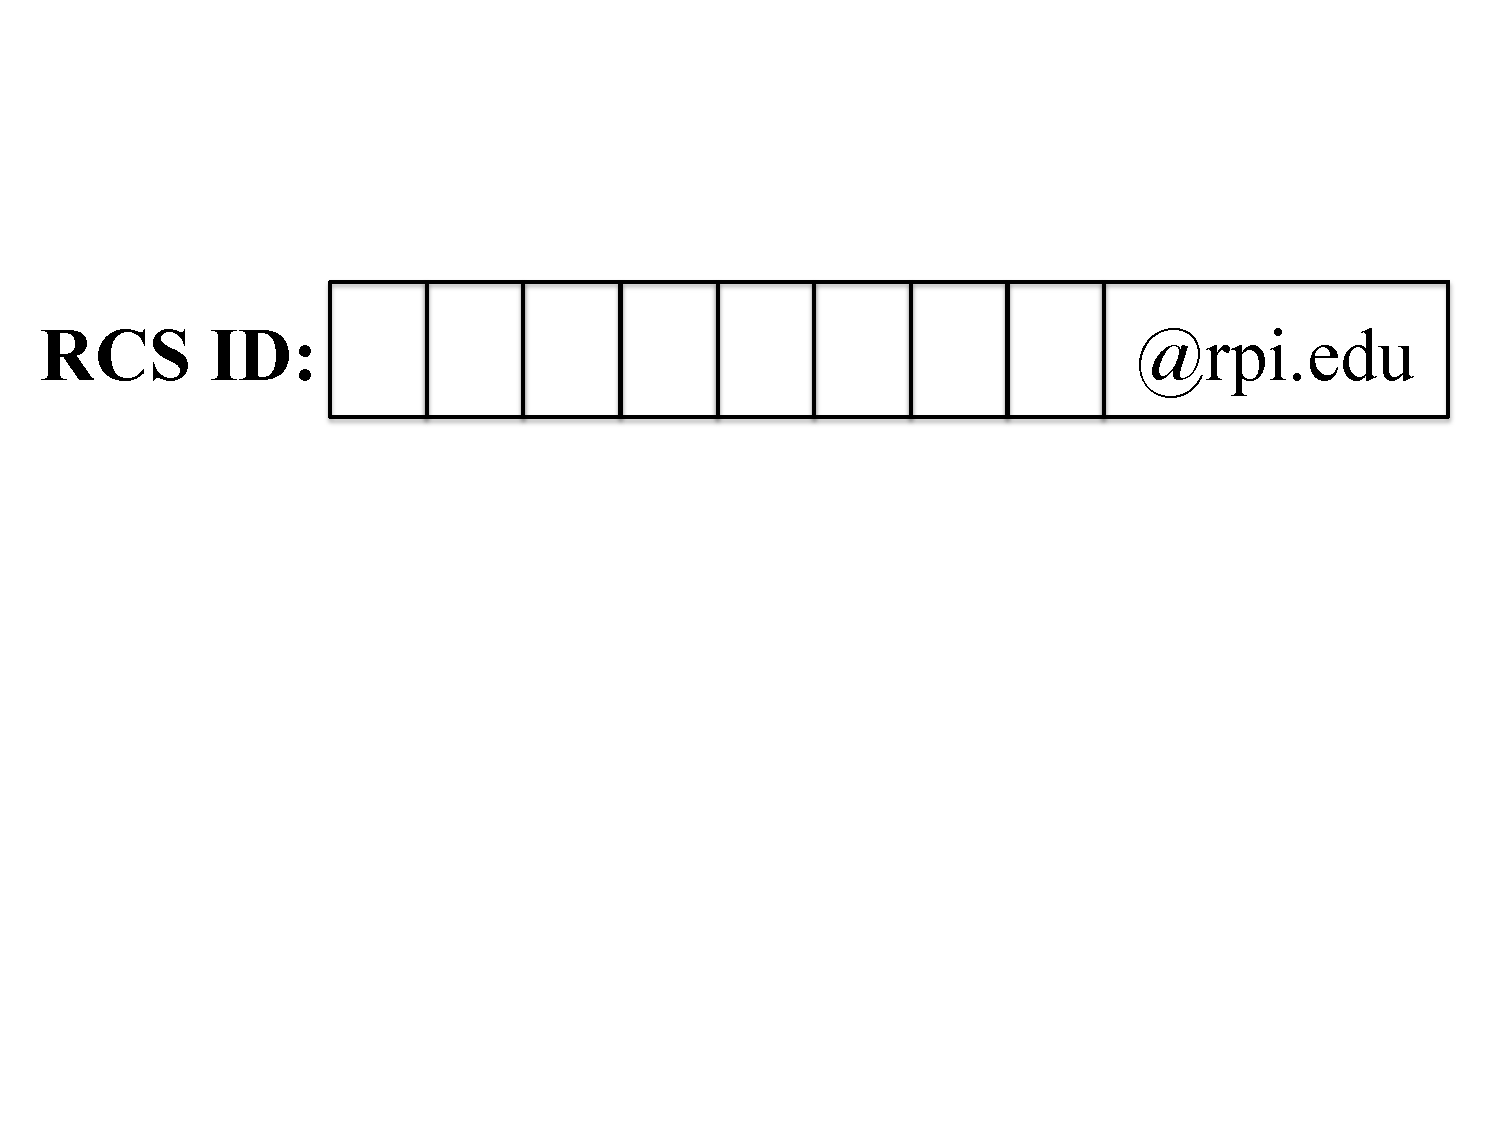
\includegraphics[height=0.5in]{boxes}
}

%%  \begin{tabular}{|p{0.1in}|p{0.1in}|p{0.1in}|p{0.1in}|p{0.1in}|p{0.1in}|p{0.1in}|p{0.1in}|l|}
%%    \hline \\
%%   & & & & & & & & \textbf{\large @rpi.edu} \\
%%  \hline
%%  \end{tabular} 
%%  
%%  \end{tabular}

\bigskip

\textbf{\Large RIN\#:} \underline {\hspace{1.5in}}  

\vspace*{0.4in}
{\large\bf Honor pledge: On my honor I have neither given
nor received aid on this exam.}

\vspace*{0.1in}
{\large\bf Please sign here to indicate that you agree with the honor pledge: \underline {\hspace{1.5in}}}
\end{center}

\vspace*{.45in} 

{\large\bf Instructions:}
\begin{itemize}
%%\item You have 90 minutes to complete this test.
\item Clearly print your name, RCS ID (in all caps.) and your RIN at the top of your exam.
\item This test is open book, open notes and open computer. You {\textbf may not} use the internet. Please turn off your wifi.
%%\item You must {\bf have your Student ID} and you must be seated in the {\bf correct section}. Failure will incur a 
%%{\bf 20 point penalty for each infraction.} If you are unsure if you
%%are in the right section, please see a proctor
%%before the exam starts.
%%\item You may use only one double-sided crib sheet.
%% Put your name and your rcs id on it and turn it in 
%%at the end of the exam.  Otherwise, put
%%  away all books, laptop computers, and electronic devices.
%%\item Please read each question carefully several times before
%%  beginning to work.
%%\item In all the questions, your output must match exactly the given
%%  output (do not insert additional spaces if they are not in the
%%  output).
%%\item We generally will not answer questions except when there is a
%%  glaring mistake or ambiguity in the statement of a question.
%%\item Except for problem 2, there are no Python syntax errors anywhere
%%  on this test. 
%%\item Unless otherwise stated, you may use any valid Python technique to solve any problem.
%%\item Please state clearly any assumptions that you have to make in
%%  interpreting a question.
\item There are \textbf{7 questions} on this test worth a total of
  \textbf{95 points}.
%%\item When you are finished with this test please turn it into one of
%%  the proctors along with your crib sheet.
%%  After you show the proctor your student id you will be free to leave
%%  the exam room.
\end{itemize}


\newpage

%%%%%%%%%%%%%%%%%%%%%%%%%%%%%%%%%%%%%%%%%%%%%%%%%%%%%%%%%%%%%%%%%%%%%%%%
\fi
%%%%%%%%%%%%%%%%%%%%%%%%%%%%%%%%%%%%%%%%%%%%%%%%%%%%%%%%%%%%%%%%%%%%%%%%

\begin{enumerate}

\item Short answers (18 pts)

\begin{enumerate}
	\item Richard Stallman defines free software as possessing four essential freedoms. Please list them below. (12 pts)

\beginanswers
\begin{itemize}
\item Freedom 0) Freedom to run the program for any purpose
\item Freedom 1) Freedom to study the program how it works and change to your likes (Access to the source code is a precondition)
\item Freedom 2) Freedom to distribute copies to others so that they can benefit
\item Freedom 3) Freedom to distribute modified versions of the code so that others can benefit from your contributions.
\end{itemize}
\else
	\begin{enumerate}
	\item 
	\bigskip
	\bigskip
	\item
	\bigskip
	\bigskip
	\item 
	\bigskip
	\bigskip
	\item
	\bigskip
	\bigskip
\end{enumerate}
\fi
	\bigskip
	\bigskip

	\item Open source licenses generally fall into two basic types: Copyleft and Permissive. Please  define Copyleft and Permissive licenses below. (6 pts)
	\begin{enumerate}
		\item The characteristics of a Copyleft license are:
		\bigskip
		\bigskip
		\bigskip
		\bigskip
		\item The characteristics of a Permissive license are:
		\bigskip
		\bigskip
		\bigskip
		\bigskip
	\end{enumerate}

\end{enumerate}

\item Please indicate whether each of the following licenses or licensing scenarios results in a  permissive, copyleft, proprietary or public domain (12 points):
\begin{enumerate}
\item Licensed with GPL:
\bigskip
\bigskip
\item Licensed with BSD:
\bigskip
\bigskip
\item An integration of two open source projects one licensed copyleft and the other licensed permissive:
\bigskip
\bigskip
\item No license:
\bigskip
\bigskip

\end{enumerate}

\item For each question below, circle the best answer (12 pts)
\begin{enumerate}
	\item Which command shows you a summary of all commits into a git repository?
	\begin{enumerate}
		\item git branch
		\item git status
		\item git checkout newbranch
		\item git log
	\end{enumerate}
\newpage
 	\item Literate programming:
 	\begin{enumerate}
 		\item Is well structured code with minimal comments
 		\item Cannot express complicated algorithms
 		\item Mixes code and comments in an easily human readable format
 		\item Is a failed development methodology
 	\end{enumerate}
 	\item Open or Free software:
 	\begin{enumerate}
 		\item Cannot be used for a commercial purpose
 		\item Can be redistributed either for free or for a fee
 		\item Can be sold, but only for the nominal cost of the media used to store it
 		\item Must be maintained by unpaid volunteers
 	\end{enumerate}
 	\item It is a good idea when selecting an open source license to:
	\begin{enumerate}
		\item Go to an authority such as the OSI and pick an approved license
		\item Create a new license from scratch because it is unlikely that an existing license would meet your needs
		\item Just place the code in a public repository. Easily available code is the same as open
		\item Take an existing, approved license and modify to better represent your unique personality
	\end{enumerate}
\end{enumerate}

\item Give a sequence of git commands to accomplish the following (you can assume that you are always working on the ``master'' branch'') (15 pts):
\begin{enumerate}
	\item Create a new git repository on your local machine.
	\item Assume you have a new file ``foo.txt'' in your local directory. Add this file to your repository.
	\item Set up your repository to communicate with a public repository at ``https://www.mypublicrepository/public.git''
	\item Send your changes to the public repository
	\item Assume someone else makes changes to the repository. Add the changes in the public repository into your local version. 
\end{enumerate}
\bigskip
Write git commands below:

\hspace*{-0.4in}\framebox(540,300){}
\newpage

\item Write markdown to duplicate the document below. You can assume the photo name is ``photo.jpg'' (15 pts):
\begin{figure}[h]
\centering
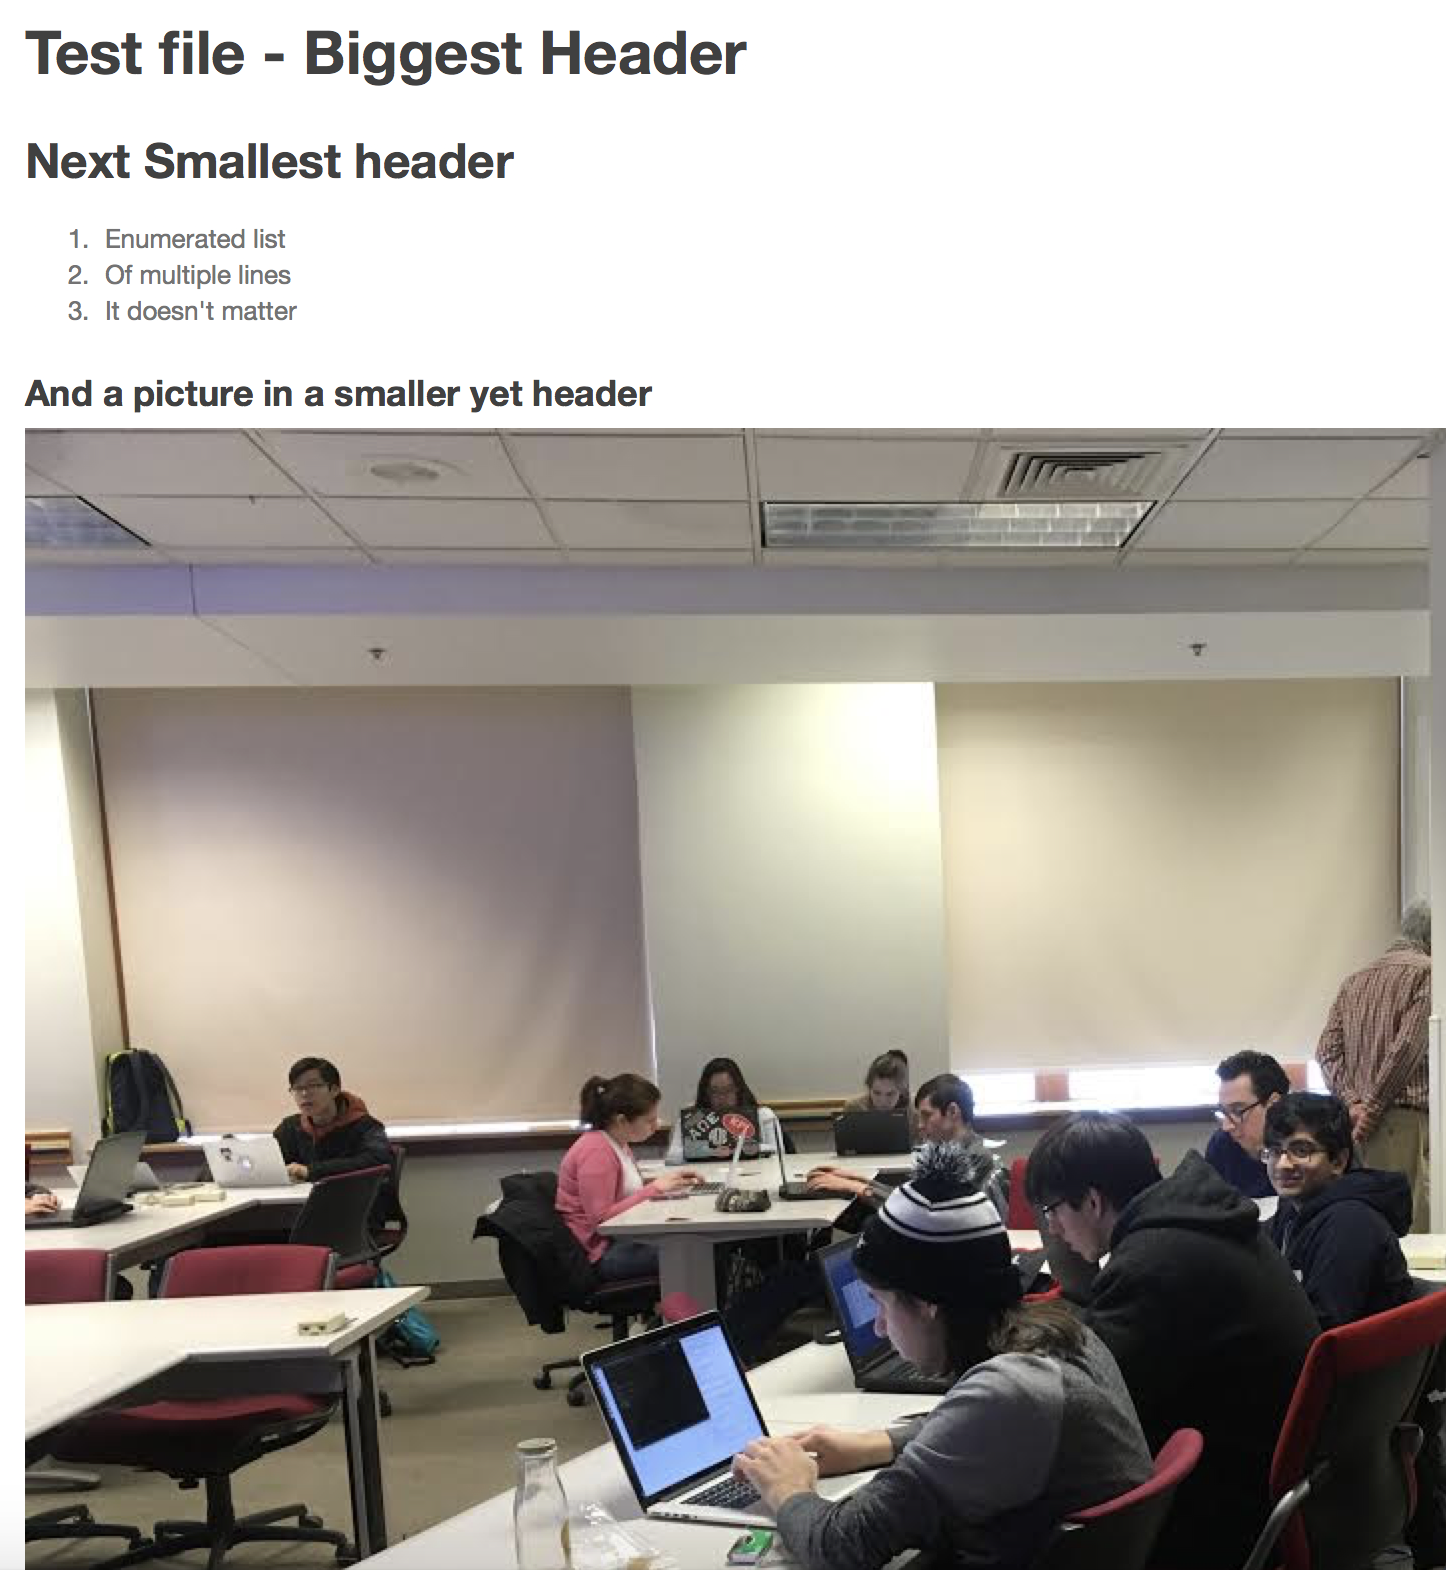
\includegraphics[width=0.7\linewidth]{./test_markdown}
\label{fig:testmarkdown}
\end{figure}

\bigskip
Write Markdown commands below:

\hspace*{-0.4in}\framebox(540,200){}
\newpage


\item Assume you have 3 source files a main file ``prog.c'' and two additional files``f1.c'', and ``f2.c'' containing code that ``prog'' depends upon. Write a Makefile that creates object files for all 3 sources, creates a library containing the code from ``f1.c'' and ``f2.c'', and then appropriately creates an executable named ``prog.exe''. Make sure your Makefile contains appropriate ``all'' and ``clean'' targets. (15 pts):
\bigskip

Write your Makefile below:

\hspace*{-0.4in}\framebox(540,275){}

\item Repeat the previous exercise for CMake.  (8 pts):
\bigskip

Write your CMakeLists.txt file below:

\hspace*{-0.4in}\framebox(540,275){}


\end{enumerate}
\end{document}

